% ==================================================================
% Graham Pellegrini — CV in LaTeX (two‑column with right sidebar)
% Save as main.tex. Compile with xelatex (recommended) or pdflatex.
% ==================================================================
\documentclass[11pt,a4paper]{article}

% ---------- Encoding & Fonts ----------
\usepackage[utf8]{inputenc}
\usepackage[T1]{fontenc}
\usepackage{lmodern}
\usepackage{microtype}
\usepackage{ragged2e} % for \justifying in sidebar

% ---------- Graphics & Color ----------
\usepackage{graphicx}
\usepackage[dvipsnames]{xcolor}
\usepackage{tikz}
\usepackage{fontawesome5}

% ---------- Layout ----------
\usepackage[a4paper,top=0cm,left=1.6cm,right=1.6cm,bottom=1.6cm,includefoot]{geometry}
\usepackage{paracol}            % two-column layout with independent flows
\columnratio{0.68}              % main : sidebar ratio (approx like your old CV)
\setlength{\columnsep}{0.9cm}  % space between columns
\setlength{\columnseprule}{0.6pt} % vertical divider rule between columns

\usepackage{enumitem}
\setlist[itemize]{leftmargin=1.2em,itemsep=0.2em,topsep=0.2em}
\usepackage{tabularx}
\usepackage{array}
\usepackage{titlesec}
\usepackage[hidelinks]{hyperref}

% ---------- Styling helpers ----------
\definecolor{accent}{HTML}{2E86AB}   % tweak to taste
\definecolor{text}{HTML}{222222}
\definecolor{muted}{HTML}{666666}
\definecolor{bannerbg}{HTML}{5CB3D6}  % Light blue for header
\definecolor{bannertext}{HTML}{FFFFFF}

\newcommand{\name}[1]{\textbf{\Large #1}}
\newcommand{\tagline}[1]{\textit{#1}}

% Section header style (clean, with underline)
\newcommand{\sectionrule}{\vspace{0.25em}\color{accent}\rule{\linewidth}{0.9pt}\vspace{0.4em}}
\titleformat{\section}{\large\bfseries\color{text}\MakeUppercase}{ }{0pt}{}
\titlespacing*{\section}{0pt}{0.6em}{0.3em}

% Sidebar section header
\newcommand{\sbheader}[1]{\vspace{0.6em}{\bfseries\color{accent}\MakeUppercase{#1}}\par\vspace{0.2em}\color{muted}\rule{\linewidth}{0.6pt}\vspace{0.3em}}

% Entry helper for dated items (Education, Experience, etc.)
\newcommand{\entry}[4]{% org, role, dates, location/notes
  \noindent\textbf{#1}\\[-1pt]
  {#2}\\[-1pt]
  \textcolor{muted}{#3}\\
  #4\par\vspace{0.6em}}

% One-line bullet list (for compact skills etc.)
\newcommand{\skilltags}[1]{\noindent\begin{tabularx}{\linewidth}{@{}>{\justifying\arraybackslash}X@{}}#1\end{tabularx}}

% Dot for contact line
\newcommand{\dotsep}{\,\textcolor{muted}{\Large\raisebox{0.2ex}{\textbullet}}\,}

% Photo command - using actual profile picture
\newcommand{\profilephoto}{%
  \begin{tikzpicture}
    \clip (0,0) circle (1.5cm);
    \node at (0,0) {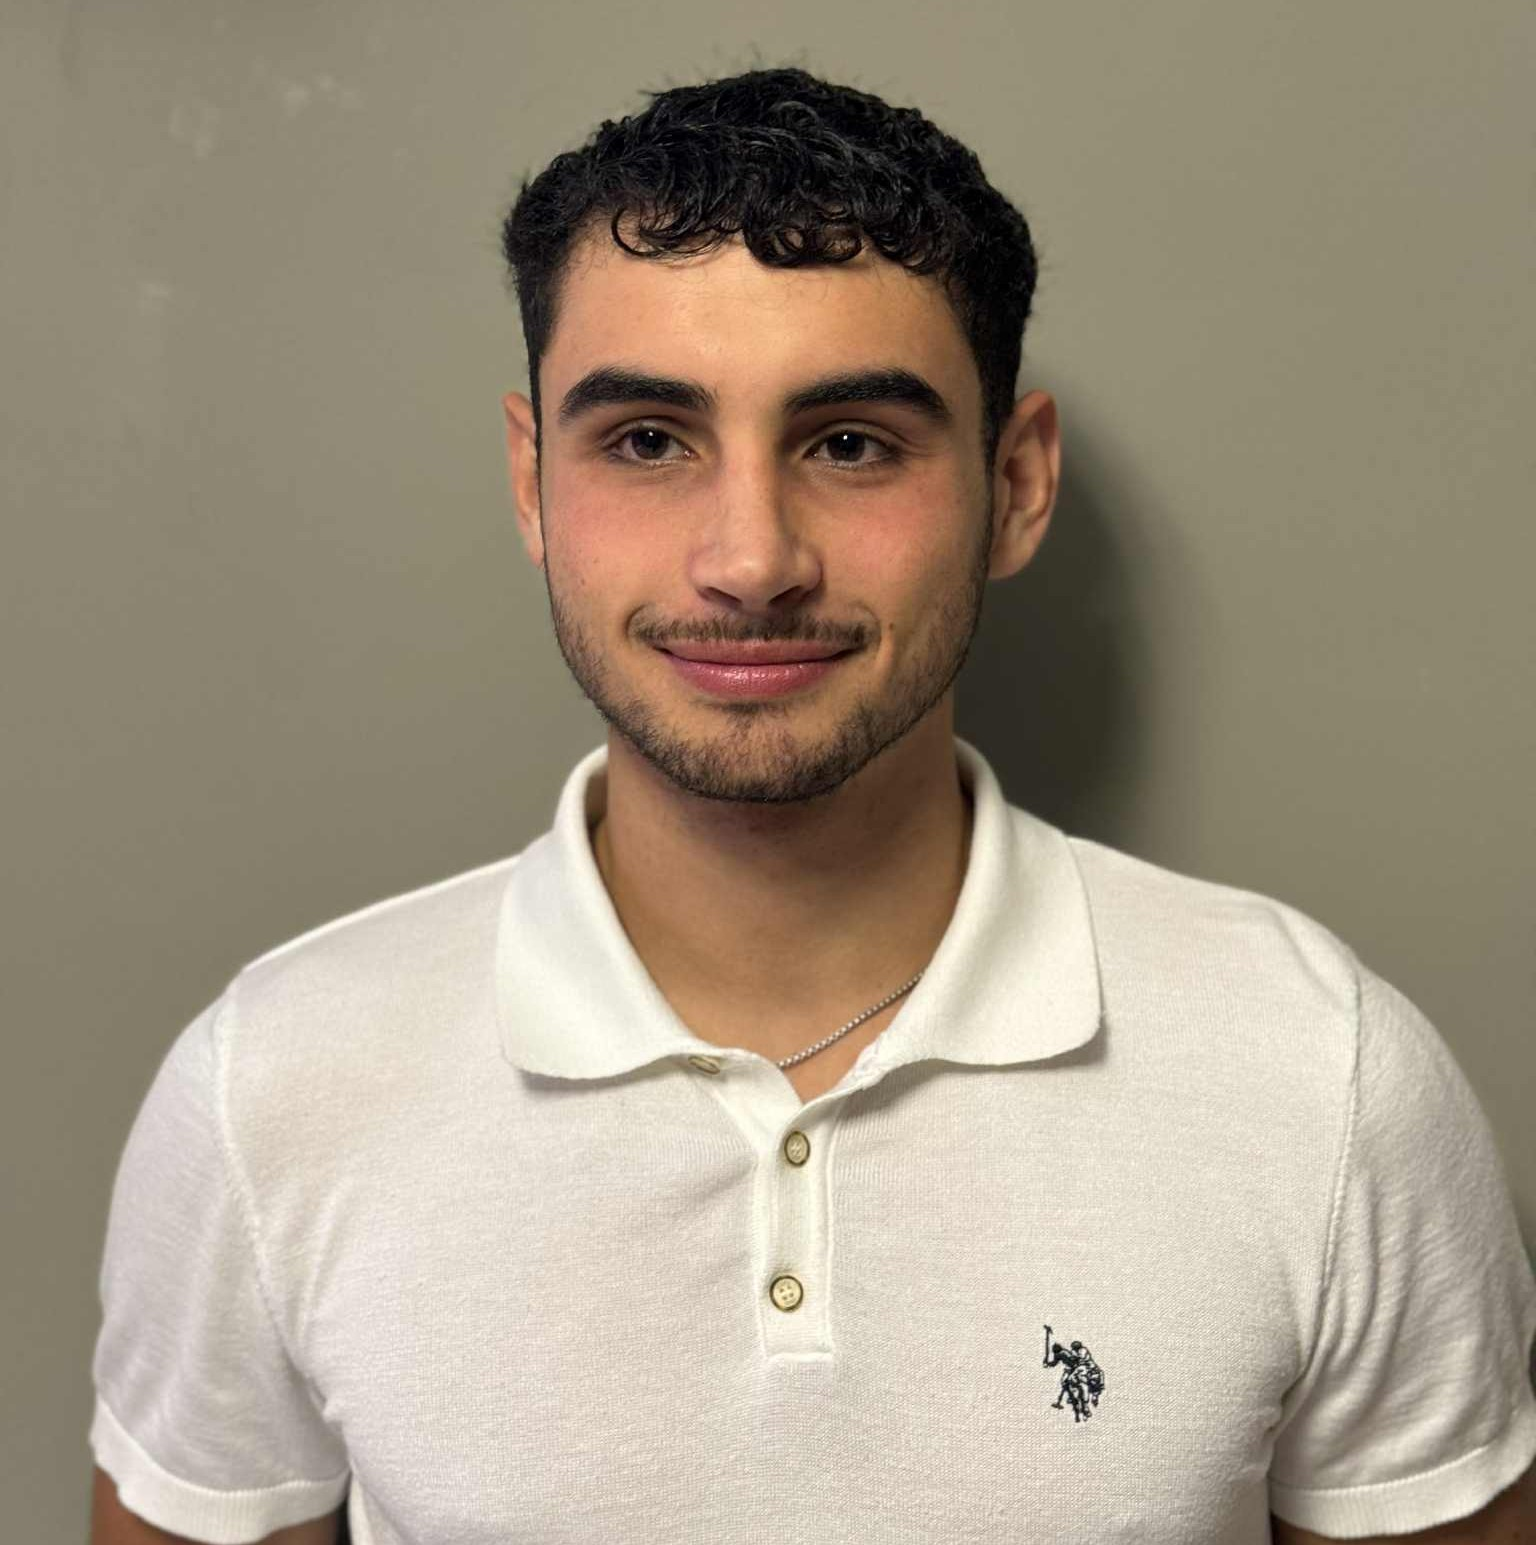
\includegraphics[width=3cm,height=3cm,keepaspectratio]{profile_picture.jpeg}};
  \end{tikzpicture}%
}

\begin{document}
\pagestyle{empty}
\color{text}
\setlength{\emergencystretch}{2em} % helps justification

% ===== Top banner with name and picture only =====
% Using tikz to create full-width header with integrated photo
\begin{tikzpicture}[remember picture,overlay]
  % Blue background banner
  \fill[bannerbg] (current page.north west) rectangle ([yshift=-3.5cm]current page.north east);
  
  % Profile picture (clipped to circle) positioned on the left side of the banner
  \begin{scope}
    \clip ([xshift=3cm,yshift=-1.75cm]current page.north west) circle (1.6cm);
    \node at ([xshift=3cm,yshift=-1.75cm]current page.north west) 
      {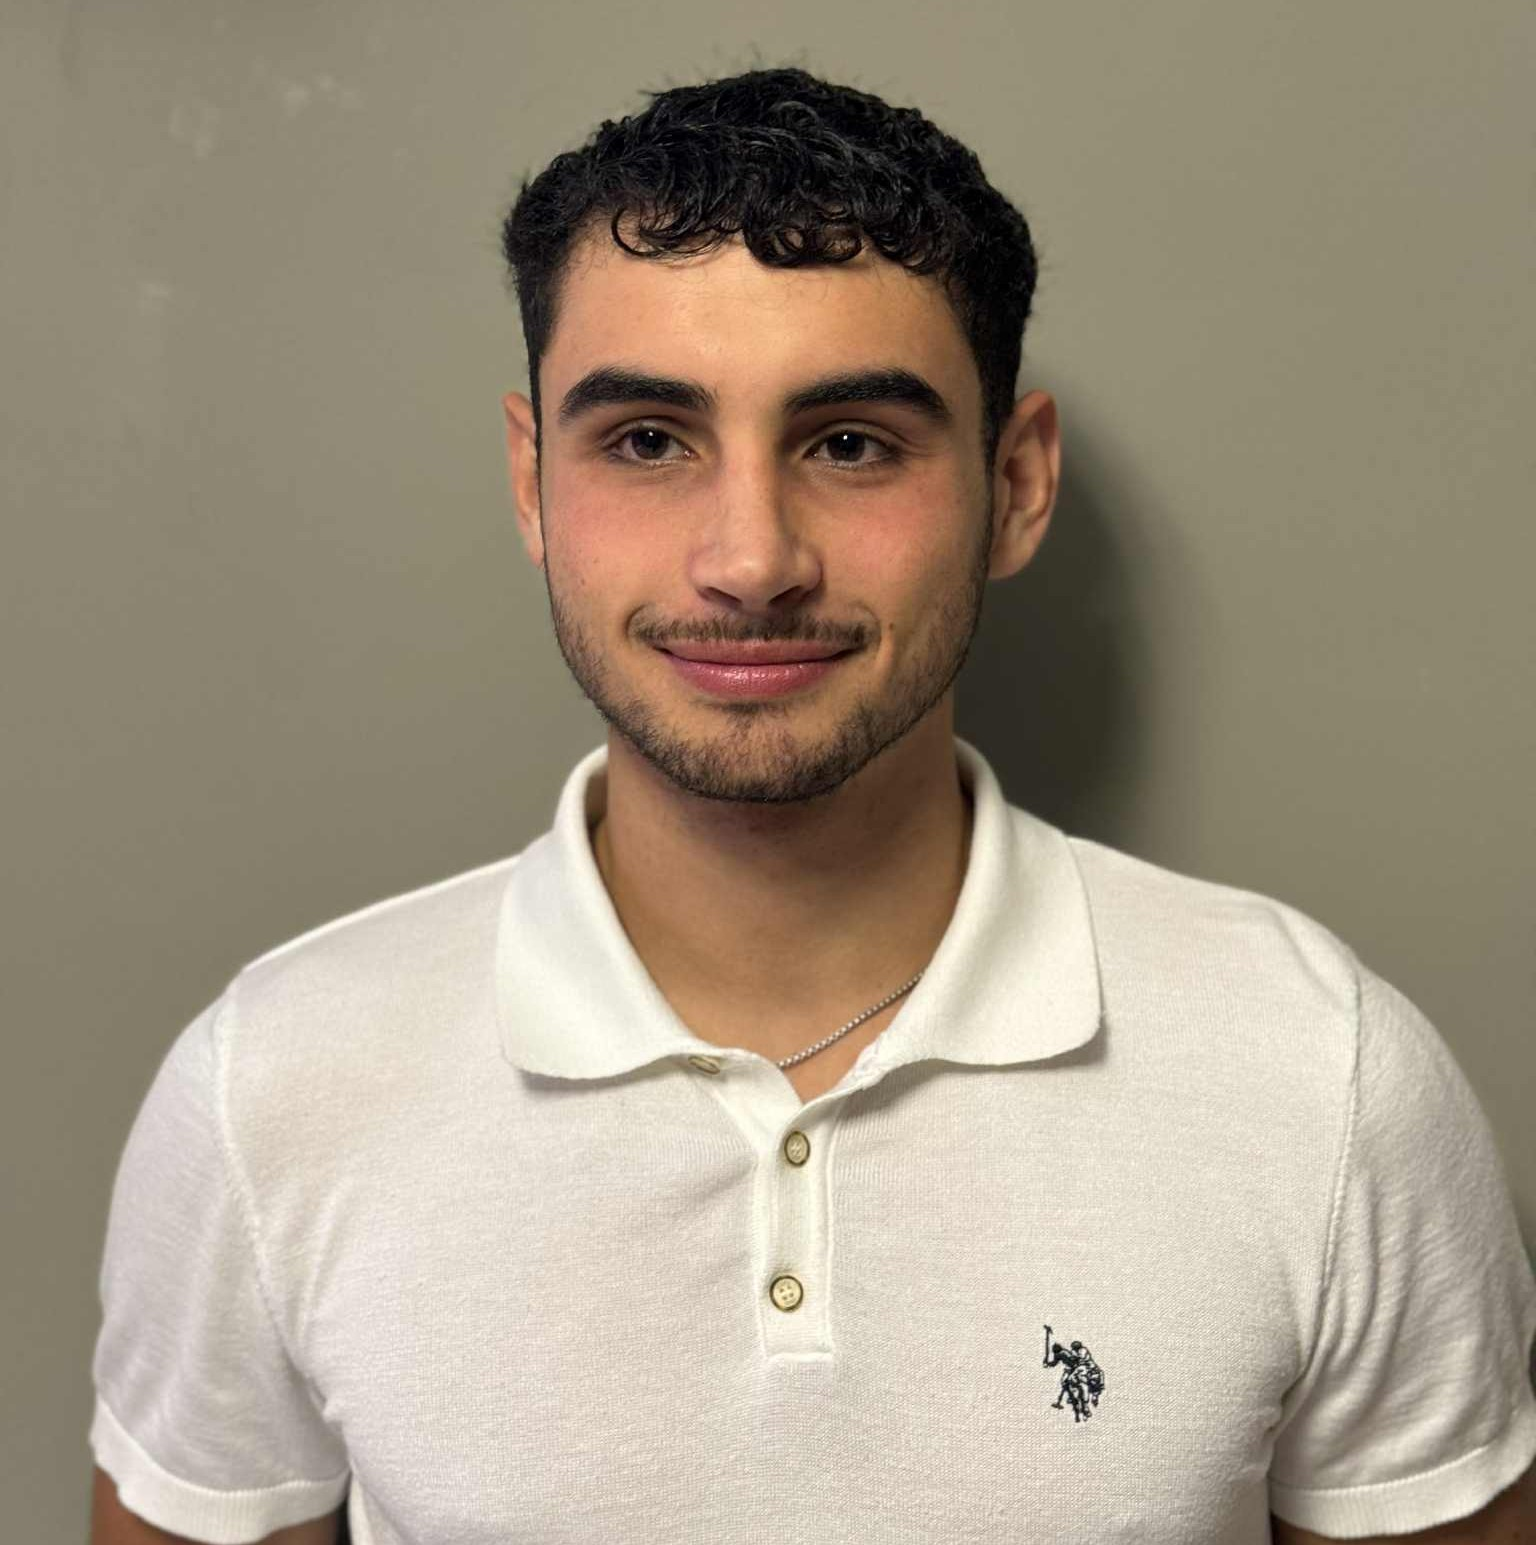
\includegraphics[width=3.2cm,height=3.2cm,keepaspectratio]{profile_picture.jpeg}};
  \end{scope}
  
  % White border around the photo
  \draw[bannertext,line width=2pt] ([xshift=3cm,yshift=-1.75cm]current page.north west) circle (1.6cm);
  
  % Name text positioned to the right of the photo
  \node[anchor=west,text=bannertext] at ([xshift=5.5cm,yshift=-1.75cm]current page.north west) 
    {\Huge\bfseries Graham Pellegrini};
\end{tikzpicture}

\vspace*{3.5cm}
\color{text}
\vspace{0.5cm}

% ===== Contact information below the header =====
\noindent
\begin{center}
\large
\href{mailto:grahammalta@gmail.com}{\faEnvelope} \hspace{1em}
\href{tel:+35699760266}{\faPhone} \hspace{1em}
\href{https://www.linkedin.com/in/graham-pellegrini-858690244/}{\faLinkedin} \hspace{1em}
\href{https://github.com/GrahamPellegrini}{\faGithub} \hspace{1em}
\faMapMarker*
\\[0.3em]
{\small 7, Hibiscus, St Julians, STJ 1573, Malta}
\end{center}
\vspace{0.8cm}

% ===== Two columns begin (vertical rule set above) =====
\begin{paracol}{2}
% --------------- Left (main) column ---------------
\section*{Profile}\sectionrule
Hardworking University student currently seeking internship opportunities to
\begin{itemize}
  \item further knowledge in the ICT sector,
  \item establish a strong work ethic and professional experience,
  \item contribute skills to facilitate company needs within a team,
  \item find a suitable place of work for years to come.
\end{itemize}

\section*{Education}\sectionrule
\entry{Matsec O-Level, St Michael's Foundation, San Gwann}{Nine subjects at Level 3}{Oct 2007 — Jun 2020}{\begin{itemize}
  \item Maltese, Religious Knowledge, English Language, English Literature, Mathematics, Physics, Accounting, Computer Studies, Economics, German (all Level 3)
\end{itemize}}

\entry{Matsec A-Level, Saint Aloysius College, Birkirkara}{Advanced \\
  \hspace*{0.75em}\textbullet\ Physics (B)\;\; \textbullet\ Pure Mathematics (B) \\
  Intermediate \\
  \hspace*{0.75em}\textbullet\ Computing (B)\;\; \textbullet\ Accounting (B)\;\; \textbullet\ English Language (C)\;\; \textbullet\ Systems of Knowledge (A)}{Oct 2020 — May 2022}{}

\entry{B.Sc. (Hons) Computer Engineering, University of Malta, Msida}{Undergraduate studies}{Oct 2022 — Present}{Currently completing 1st year.}

\section*{Extra-curricular}\sectionrule
\entry{National Athlete, Athletics Malta, Marsa}{Middle-distance sprinter (200m \& 400m)}{Mar 2019 — Present}{}
\entry{Advanced Open Water Diver, Watercolours Dive Centre, Sliema}{SSI Certifications}{Jul 2022 — Present}{\begin{itemize}
  \item Open Water Diver (SSI)
  \item Advanced Adventurer (SSI)
\end{itemize}}

\section*{Certificates}\sectionrule
\begin{itemize}
  \item Certificate of Participation, 10th Malta Mathematics Olympiad (Apr 2019)
  \item ISF World School Championships Athletics, Croatia (May 2019)
  \item U18 Athlete of the Year (2020)\;\&\; (2021)
  \item ECDL (Jun 2020)
  \item Social Responsibility Programme (Salesians Senglea) completion (Jun 2022)
  \item Advanced and Open Water Diver (Aug 2022)
  \item U20 300m National Record Holder (Feb 2023)
\end{itemize}

\section*{Courses}\sectionrule
\entry{Basic Track on Quantum Computing, Qalypso Summer School}{}{Sep 2022}{}

% --------------- Switch to right (sidebar) column ---------------
\switchcolumn
\footnotesize\justifying  % Using footnotesize instead of small for smaller text

\sbheader{Details}
\begin{tabularx}{\linewidth}{@{}>{\bfseries}p{3.2cm}>{\justifying\arraybackslash}X@{}}
Nationality & Maltese \\
Date / place of birth & 23/10/2004, Piet\'a \\
\end{tabularx}

\sbheader{Links}
\noindent LinkedIn: \href{https://www.linkedin.com/in/graham-pellegrini-858690244/}{graham-pellegrini-858690244} \par
\noindent Facebook: \href{https://www.facebook.com/GrahamPelle2004}{GrahamPelle2004} \par
\noindent Instagram: \href{https://www.instagram.com/grahampelle_/}{@grahampelle\_}

\sbheader{Skills}
\skilltags{Inquisitive learner \;\textbullet\; Strong with computers \& tech \\
Developed communication \;\textbullet\; Critical thinker \\
Fast learner \;\textbullet\; Effective time management \\
Team collaboration}

\sbheader{Hobbies}
\skilltags{Diving \;\textbullet\; Athletics \;\textbullet\; Computer tinkering}

\sbheader{Languages}
\skilltags{English (fluent) \;\textbullet\; Maltese (fluent) \;\textbullet\; German (conversational)}

\end{paracol}

\end{document}
